
\subsubsection{補正手法の設計}


% TODO: 精度向上という文が気になる.
PDRによる位置推定の精度を向上させるため本ライブラリは複数の補正手法を
組み合わせた設計を採用している.
これらの補正手法を統合的に扱うために,TrajectoryCorrectrorクラスを中心とした設計を提供している.
図\ref{fig:corrector-class}に示すように,補正処理はTrajectoryCorrector,
DriftCorrector,MapMatchCorrector,WirelessSignalCorrectorの4つの主要なクラスから構成されており,
それぞれが特定の補正機能を担当している.各補正クラスは独立して実装されており,
TrajectoryCorrectorを介して緩やかに結合され,保守性と拡張性を実現している.

\begin{figure}[H]
    \centering
    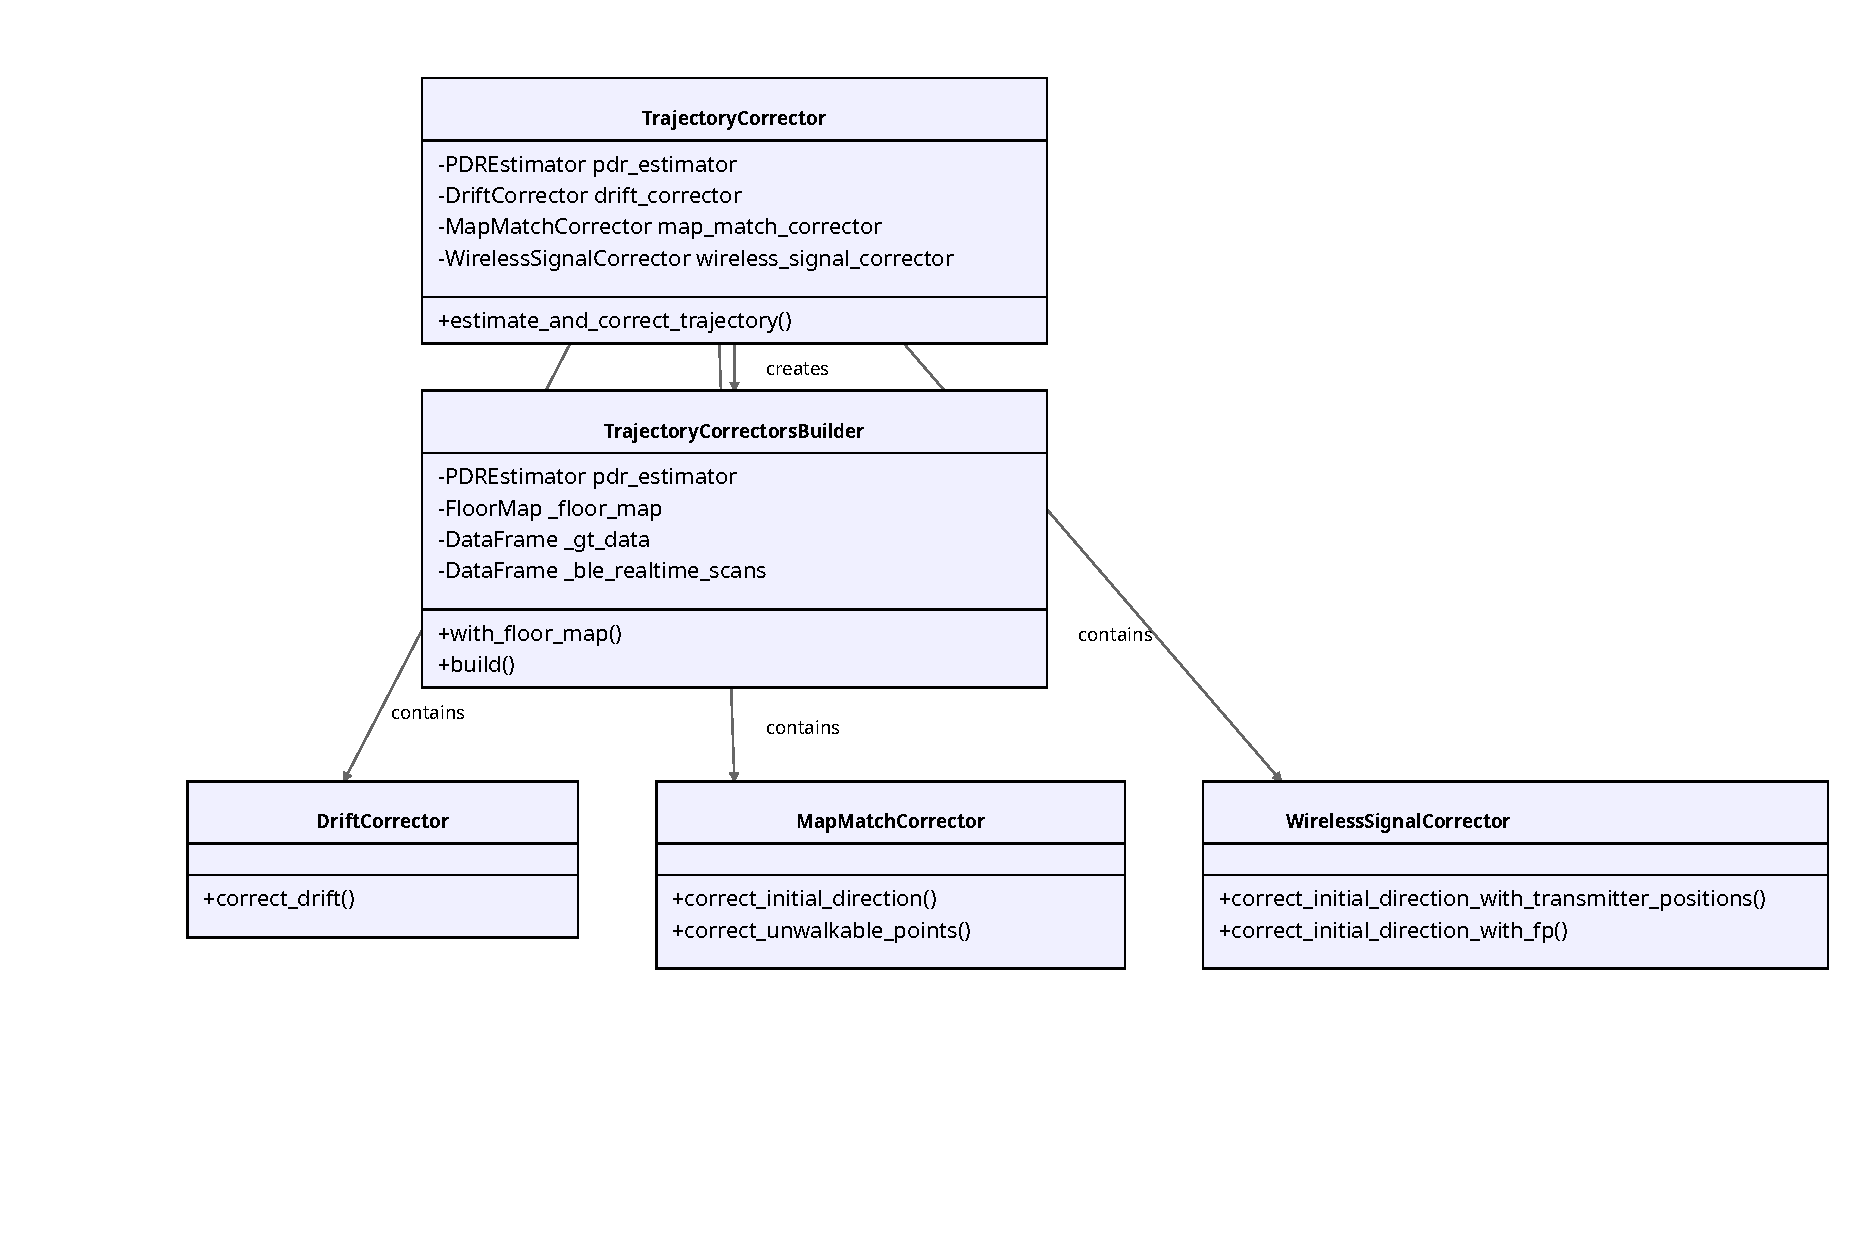
\includegraphics[width=\linewidth]{../image/trajectory_corrector.pdf}
    \caption{補正における主要クラス設計}
    \label{fig:corrector-class}
\end{figure}

補正処理の柔軟な設定を実現するため,TrajectoryCorrectorクラスはBuilderパターンを採用している.
Builderパターンは複雑なオブジェクトの生成過程を抽象化し,段階的な構築を可能にする設計パターンである.
このパターンの採用により補正処理の設定に必要な多数のパラメータを直感的に設定でき,
また設定の順序や組み合わせによる問題を回避できる.
Listing\ref{lst:trajectory-corrector}にその例を示す.
利用者はwith\_floor\_map()やwith\_wireless\_signal()などのメソッドチェーンを通じて,必要な補正手法を宣言的に指定できる. 
フロアマップと電波情報が利用可能な環境では両方の補正を組み合わせ,
フロアマップのみが利用可能な環境ではMapMatchCorrectorによる補正のみを指定するなど,
環境に応じた最適な補正手法の選択が可能となる.
また各補正クラスは単体でも使用可能であり特定の補正処理のみを実行したい場合は直接該当するクラスを利用できる.

\begin{lstlisting}[caption={TrajectoryCorrectorの使用例},label=lst:trajectory-corrector,float=h]
# フロアマップのみを使用する場合
corrector = TrajectoryCorrector.builder(pdr_estimator)
    .with_floor_map(floor_map)
    .build()

# フロアマップと電波情報を組み合わせる場合
corrector = TrajectoryCorrector.builder(pdr_estimator)
    .with_floor_map(floor_map)
    .with_wireless_signal(ble_scans beacon_positions)
    .build()
\end{lstlisting}

この設計の特徴は新たな補正手法の追加が容易である点にある.
例えば磁気フィンガープリントを用いた補正手法を追加する場合
MagneticCorrectorクラスを新規作成し,
TrajectoryCorrectorsBuilderに対応するメソッドを
追加するだけで良い.
この際既存の補正クラスのコードを変更する必要がないためシステムの安定性を保ちながら機能を拡張できる.
また各補正手法は独立して実装されているため,個々の手法の改良やバグ修正も他の機能に影響を与えず実装できる.

% TODO:フローよりシーケエンスの方がいいのか?
図\ref{fig:corrector-sequence}はBuilderパターンを用いた
TrajectoryCorrectorクラスの生成と軌跡補正処理のフロー図である.
TrajectoryCorrectorsBuilderを通じて必要な補正手法を指定し,buildメソッド
によってTrajectoryCorrectorのインスタンスを生成する.
その後estimate\_and\_correct\_trajectoryメソッドを呼び出すと指定された補正手法が順次適用され,最終的な補正軌跡が得られる.
この処理フローにより複数の補正手法を組み合わせた位置推定が可能となっている.

% TODO:画像の下に空白がありすぎる
\begin{figure}[H]
    \centering
    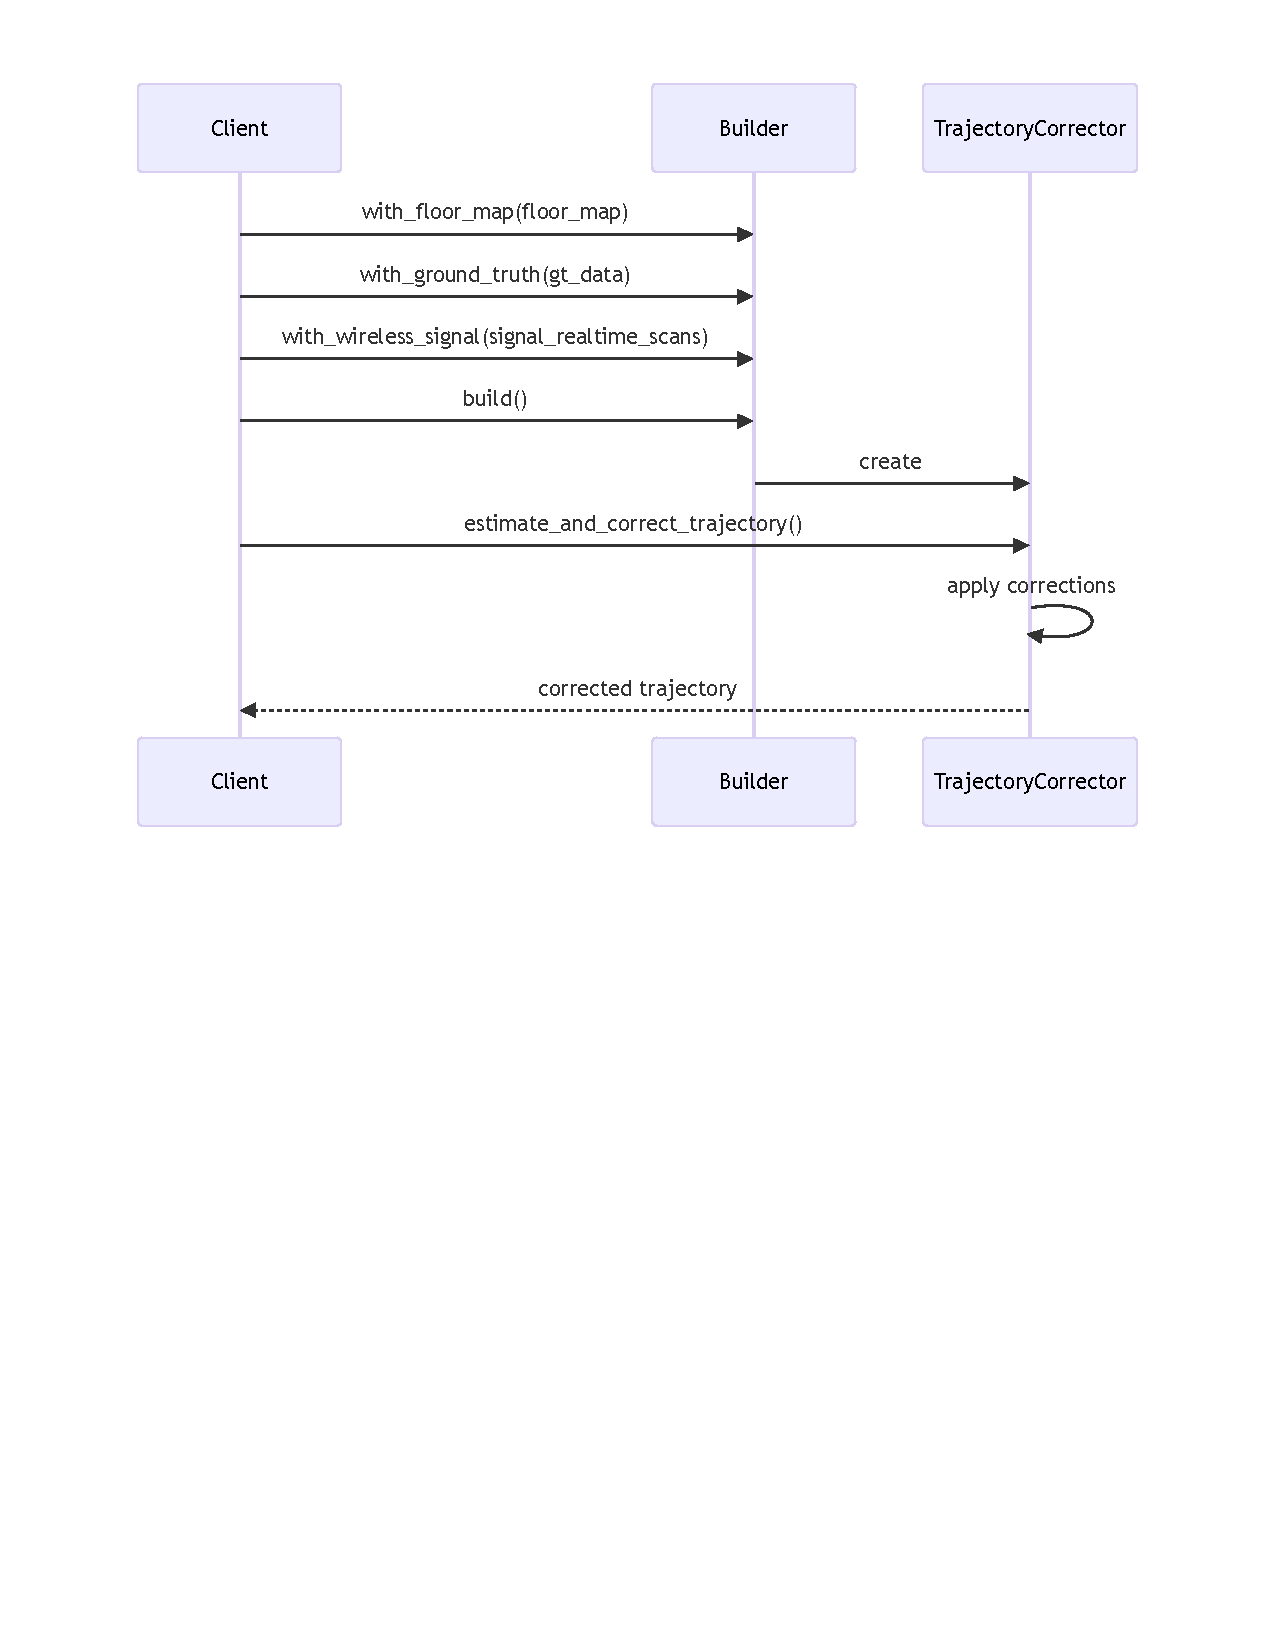
\includegraphics[width=\linewidth]{../image/corrector-flow-diagram.pdf}
    \caption{Builderパターンを用いたTrajectoryCorrectorクラスの生成と軌跡補正処理のフロー}
    \label{fig:corrector-sequence}
\end{figure}
